\documentclass[twoside,a4paper,10]{book}
\usepackage{graphicx}
\usepackage{hyperref}
\usepackage{amsmath}
\usepackage{amssymb}
\usepackage{textcomp}
\usepackage[utf8]{inputenc}
\usepackage[polish]{babel}
\usepackage[T1]{fontenc}
\usepackage{standalone}
\usepackage{array}
% pakiet stosowany do url'i w bibliografii, zamienia odnośniki na ładnie sformatowane
\usepackage{url}


% pakiety służące do numerowania i tworzenia algorytmów
\usepackage{algorithmic}
\usepackage{algorithm}
% redefinicja etykiety nagłówkowej listy algorytmów, domyślna jest po angielsku
\renewcommand{\listalgorithmname}{Spis algorytmów}

\usepackage[section]{placeins}
\usepackage{pdfpages}

% pakiet do wyliczania skali, przydatny przy dużych obrazkach
\usepackage{pgf}
% pakiet służący do automatycznego sortowania odnośników do bibliografii
\usepackage[sort]{natbib}

% tworzenie listingów
\usepackage{listings}
% tworzenie figur wewnątrz figur
\usepackage{subfig}
% do automatycznego skracania nazw rozdziałów i podrozdziałów używanych w nagłówkach strony by mieściły się w jednej linii
\usepackage[fit]{truncate}
% fancyhdr - ładne nagłówki, definicja wyglądu nagłówka, numery stron będą umieszczane w nagłówku po odpowiedniej stronie
\usepackage{fancyhdr}
\pagestyle{fancy}
\renewcommand{\chaptermark}[1]{\markboth{#1}{}}
\renewcommand{\sectionmark}[1]{\markright{\thesection\ #1}}



\fancyhf{}
\fancyhead[LE,RO]{\bfseries\thepage}
% tutaj ograniczamy szerokość pola w nagłówku zawierającego nazwę rozdziału/podrozdziału do 95% szerokości strony
% redefinicja sposobu prezentacji nazw domyślnie wypisywanych wielkimi literami (np. domyślnie w nagłówku Spis treści będzie miał postać SPIS TREŚCI)
% Uwaga! to może popsuć wielkie litery w ogóle! Jak coś nie działa należy usunąć \nouppercase{} z poniższych definicji
\fancyhead[LO]{\nouppercase{\bfseries{\truncate{.95\headwidth}{\rightmark}}}}
\fancyhead[RE]{\nouppercase{\bfseries{\truncate{.95\headwidth}{\leftmark}}}}
\renewcommand{\headrulewidth}{0.5pt}
\renewcommand{\footrulewidth}{0pt}

% definicja typu prostego wymagana przez pierwsze strony rozdziałów itp.
% powyższe reguły niestety tych stron nie dotyczą, gdyż Latex automatycznie przełącza je pomiędzy fancy a plain
% w tym wypadku eliminujemy nagłówki i stopki na stronach początkowych
\fancypagestyle{plain}{%
 \fancyhead{}
 \fancyfoot{}
 \renewcommand{\headrulewidth}{0pt}
 \renewcommand{\footrulewidth}{0pt}
}

\parskip 0.05in


% makro umożliwiające otaczanie symboli okręgami
\usepackage{tikz}
% brak justowania tekstu (bazą okręgu będzie linia tekstu)
\newcommand*\mycirc[1]{
  \begin{tikzpicture}
    \node[draw,circle,inner sep=1pt] {#1};
  \end{tikzpicture}}

% pionowe justowanie tekstu, środek okręgu pokrywa się ze środkiem tekstu
\newcommand*\mycircalign[1]{%
  \begin{tikzpicture}[baseline=(C.base)]
    \node[draw,circle,inner sep=1pt](C) {#1};
  \end{tikzpicture}}

% zmiana nazwy twierdzeń i lematów
\newtheorem{theorem}{Twierdzenie}[section]
\newtheorem{lemma}[theorem]{Lemat}

% tworzenie definicji dowodu
\newenvironment{proof}[1][Dowód]{\begin{trivlist}
\item[\hskip \labelsep {\bfseries #1}]}{\end{trivlist}}
% \newenvironment{definition}[1][Definicja]{\begin{trivlist}
% \item[\hskip \labelsep {\bfseries #1}]}{\end{trivlist}}
% \newenvironment{example}[1][Przykład]{\begin{trivlist}
% \item[\hskip \labelsep {\bfseries #1}]}{\end{trivlist}}
% \newenvironment{remark}[1][Uwaga]{\begin{trivlist}
% \item[\hskip \labelsep {\bfseries #1}]}{\end{trivlist}}

% definicja czarnego prostokąta zwyczajowo dodawanego na koniec dowodu
\newcommand{\qed}{\nobreak \ifvmode \relax \else
      \ifdim\lastskip<1.5em \hskip-\lastskip
      \hskip1.5em plus0em minus0.5em \fi \nobreak
      \vrule height0.75em width0.5em depth0.25em\fi}

% poniższymi instrukcjami można sterować co ma być numerowane a co nie i co ma być wyświetlane w spisie treści
% \setcounter{secnumdepth}{3}
% \setcounter{tocdepth}{5}

% definicja czcionki mniejszej niż tiny (domyślnie takiej małej nie ma)
\usepackage{lmodern}
\makeatletter
  \newcommand\tinyv{\@setfontsize\tinyv{4pt}{6}}
\makeatother

% definicja jeszcze mniejszej czcionki
\usepackage{lmodern}
\makeatletter
  \newcommand\tinyvv{\@setfontsize\tinyvv{3.5pt}{6}}
\makeatother

% pakiet do obsługi wielostronicowych tabel
\usepackage{longtable}
\setlength{\LTcapwidth}{\textwidth}

\usepackage[section] {placeins}

\usepackage{multirow}

\usepackage{slantsc}
\usepackage[labelsep= space]{caption}
\usepackage[font=small,labelfont=bf]{caption}
\usepackage[justification=centering]{caption}
\addto\captionspolish{\renewcommand{\figurename}{Rys.}}
\addto\captionspolish{\renewcommand{\tablename}{Tab.}}
\addto\captionspolish{\renewcommand*{\appendixpagename}{Dodatki}}
\addto\captionspolish{\renewcommand*{\appendixtocname}{Dodatki}}
\addto\captionspolish{\renewcommand*{\appendixname}{Dodatek}}

%CZCIONKA%
\usepackage{helvet}
\renewcommand{\familydefault}{\sfdefault}
\linespread{1.25}
\newcolumntype{M}[1]{>{\centering\arraybackslash}m{#1}}
\usepackage{csquotes}
\usepackage[toc,page]{appendix}
\begin{document}

\chapter{Stan wiedzy} ~\label{sec:chap1} 

\section{ Teoria ewolucji}
Teoria zaprezentowana przez uczonego przyrodnika i geologa Charlesa Darwina w 1859 w pierwszym wydaniu jego książki, \enquote{\textit{The Origin of Species}},  podsumowującej lata pracy i zebrane doświadczenia na temat rozwoju gatunków. 
W ogólności teoria ewolucji głosi, że wszystkie organizmy żywe są ze sobą spokrewnione i pochodzą od jednego wspólnego przodka. Świat istot żywych podlega ciągłym i stopniowym zmianom, dążącym do adaptacji organizmów, a wszystkie zmiany te są wynikiem doboru naturalnego.   ~\cite{darwin}
\\Teoria Darwina opiera się na pewnym zbiorze zasad  ~\cite{darwin},  ~\cite{darwinWeb}: 
\begin{itemize}
\item{   Prawo zmienności powszechnej i bezkierunkowej}\\
Wyjaśnia, iż jedynie zmienność dziedziczna ma wpływ na ewolucję. Zmienność niedziedziczna, nie wpływa na jej przebieg.
\item{  Prawo różnorodności gatunków}\\ Głosi, że gatunki dzielą się na podgatunki potomne, lub w procesie pączkowania wytwarzają innego rodzaju organizmy potomne.
\item{   Prawo walki o byt}\\ Jest to mechanizm redukujący nadmiar populacji, będący czynnikiem napędzającym proces ewolucji.  Walka o byt może się odbywać między różnymi gatunkami w układzie ofiara - drapieżnik lub w obrębie jednego gatunku w wyniku konkurencji o tę samą niszę ekologiczną. 
\item{    Prawo doboru naturalnego}
\\ Przeżywają  jedynie osobniki najlepiej przystosowane, a formy pośrednie wymierają, co prowadzi do coraz większej rozbieżności cech w następnych pokoleniach i powstania z czasem form bardzo różniących się od praprzodka i powstawania nowych gatunków.
\item{   Prawo dziedziczenia}
\\ Bezpośrednio łączy się z powyższym prawem. Osobniki słabsze, częściej padające ofiarą, mają mniejsze szanse na rozmnażanie, a co za tym idzie na przekazanie swojego zestawu cech. Powstają organizmy potomne, dziedziczące jedynie cechy od silnych osobników, które przetrwały. 
\end{itemize}
Wszystkie tezy zostały potwierdzone badaniami z dziedziny biologii molekularnej, ekologii oraz biogeografii. 
  \section{Ewolucja Organiczna}
    Ewolucja to  proces stopniowej przemiany osobników (zarówno zwierząt jak i roślin), który w ostateczności może doprowadzić do powstania nowych gatunków. Przemiana ta może dotyczyć zarówno cech morfologicznych jak i fizjologicznych. Jej istotą jest zmiana składu materiału genetycznego organizmów potomnym w stosunku do organizmów rodzicielskich. ~\cite{encyk}  
Zmiany te mogą być wynikiem różnych mechanizmów:
             \subsection{  Mutacje i zmienność rekombinacyjna }~\label{sec:mutate}
Występowanie tych dwóch mechanizmów ma charakter losowy. Zmienność rekombinacyjna jest wynikiem mieszania się materiału genetycznego, natomiast mutacje spowodowane są zmianami w obrębie jednego organizmu.
    Mutacje mogą być typu punktowego (dotyczące  jednego nukleotydu) lub obejmować większy odcinek DNA (chromosomowe). Wśród nich wyróżniamy:
\begin{itemize}
\item{substytucję, }
\item{delecję,}
\item{insercję,}
\item{tranzycję,}
\item{transwersję}
\item{inwersję, }
\item{deficjencję,}
\item{translokację. ~\cite{berkely}}
\end{itemize}

    Zmienność rekombinacyjna zachodzi dzięki zjawiskom takim jak: crossing-over, niezależna segregacja chromosomów i połączenie gamet.
           \subsubsection{ Crossing-over} 
Crossing-over, inaczej krzyżowanie,  jest zjawiskiem wymiany materiału genetycznego między chromatydami 
niesiostrzanymi chromosomów homologicznych podczas procesu mejozy. ~\cite{bioDicWeb} Schemat zachodzenia crossing-over zaprezentowano na grafice rys.~\ref{fig:crossingover}. Chromosomami homologicznymi nazywamy parę chromosomów pochodzących, po jednym, od osobników rodzicielskich. 
\begin{figure}[!h]
		\centering
		\scalebox{.8}{
		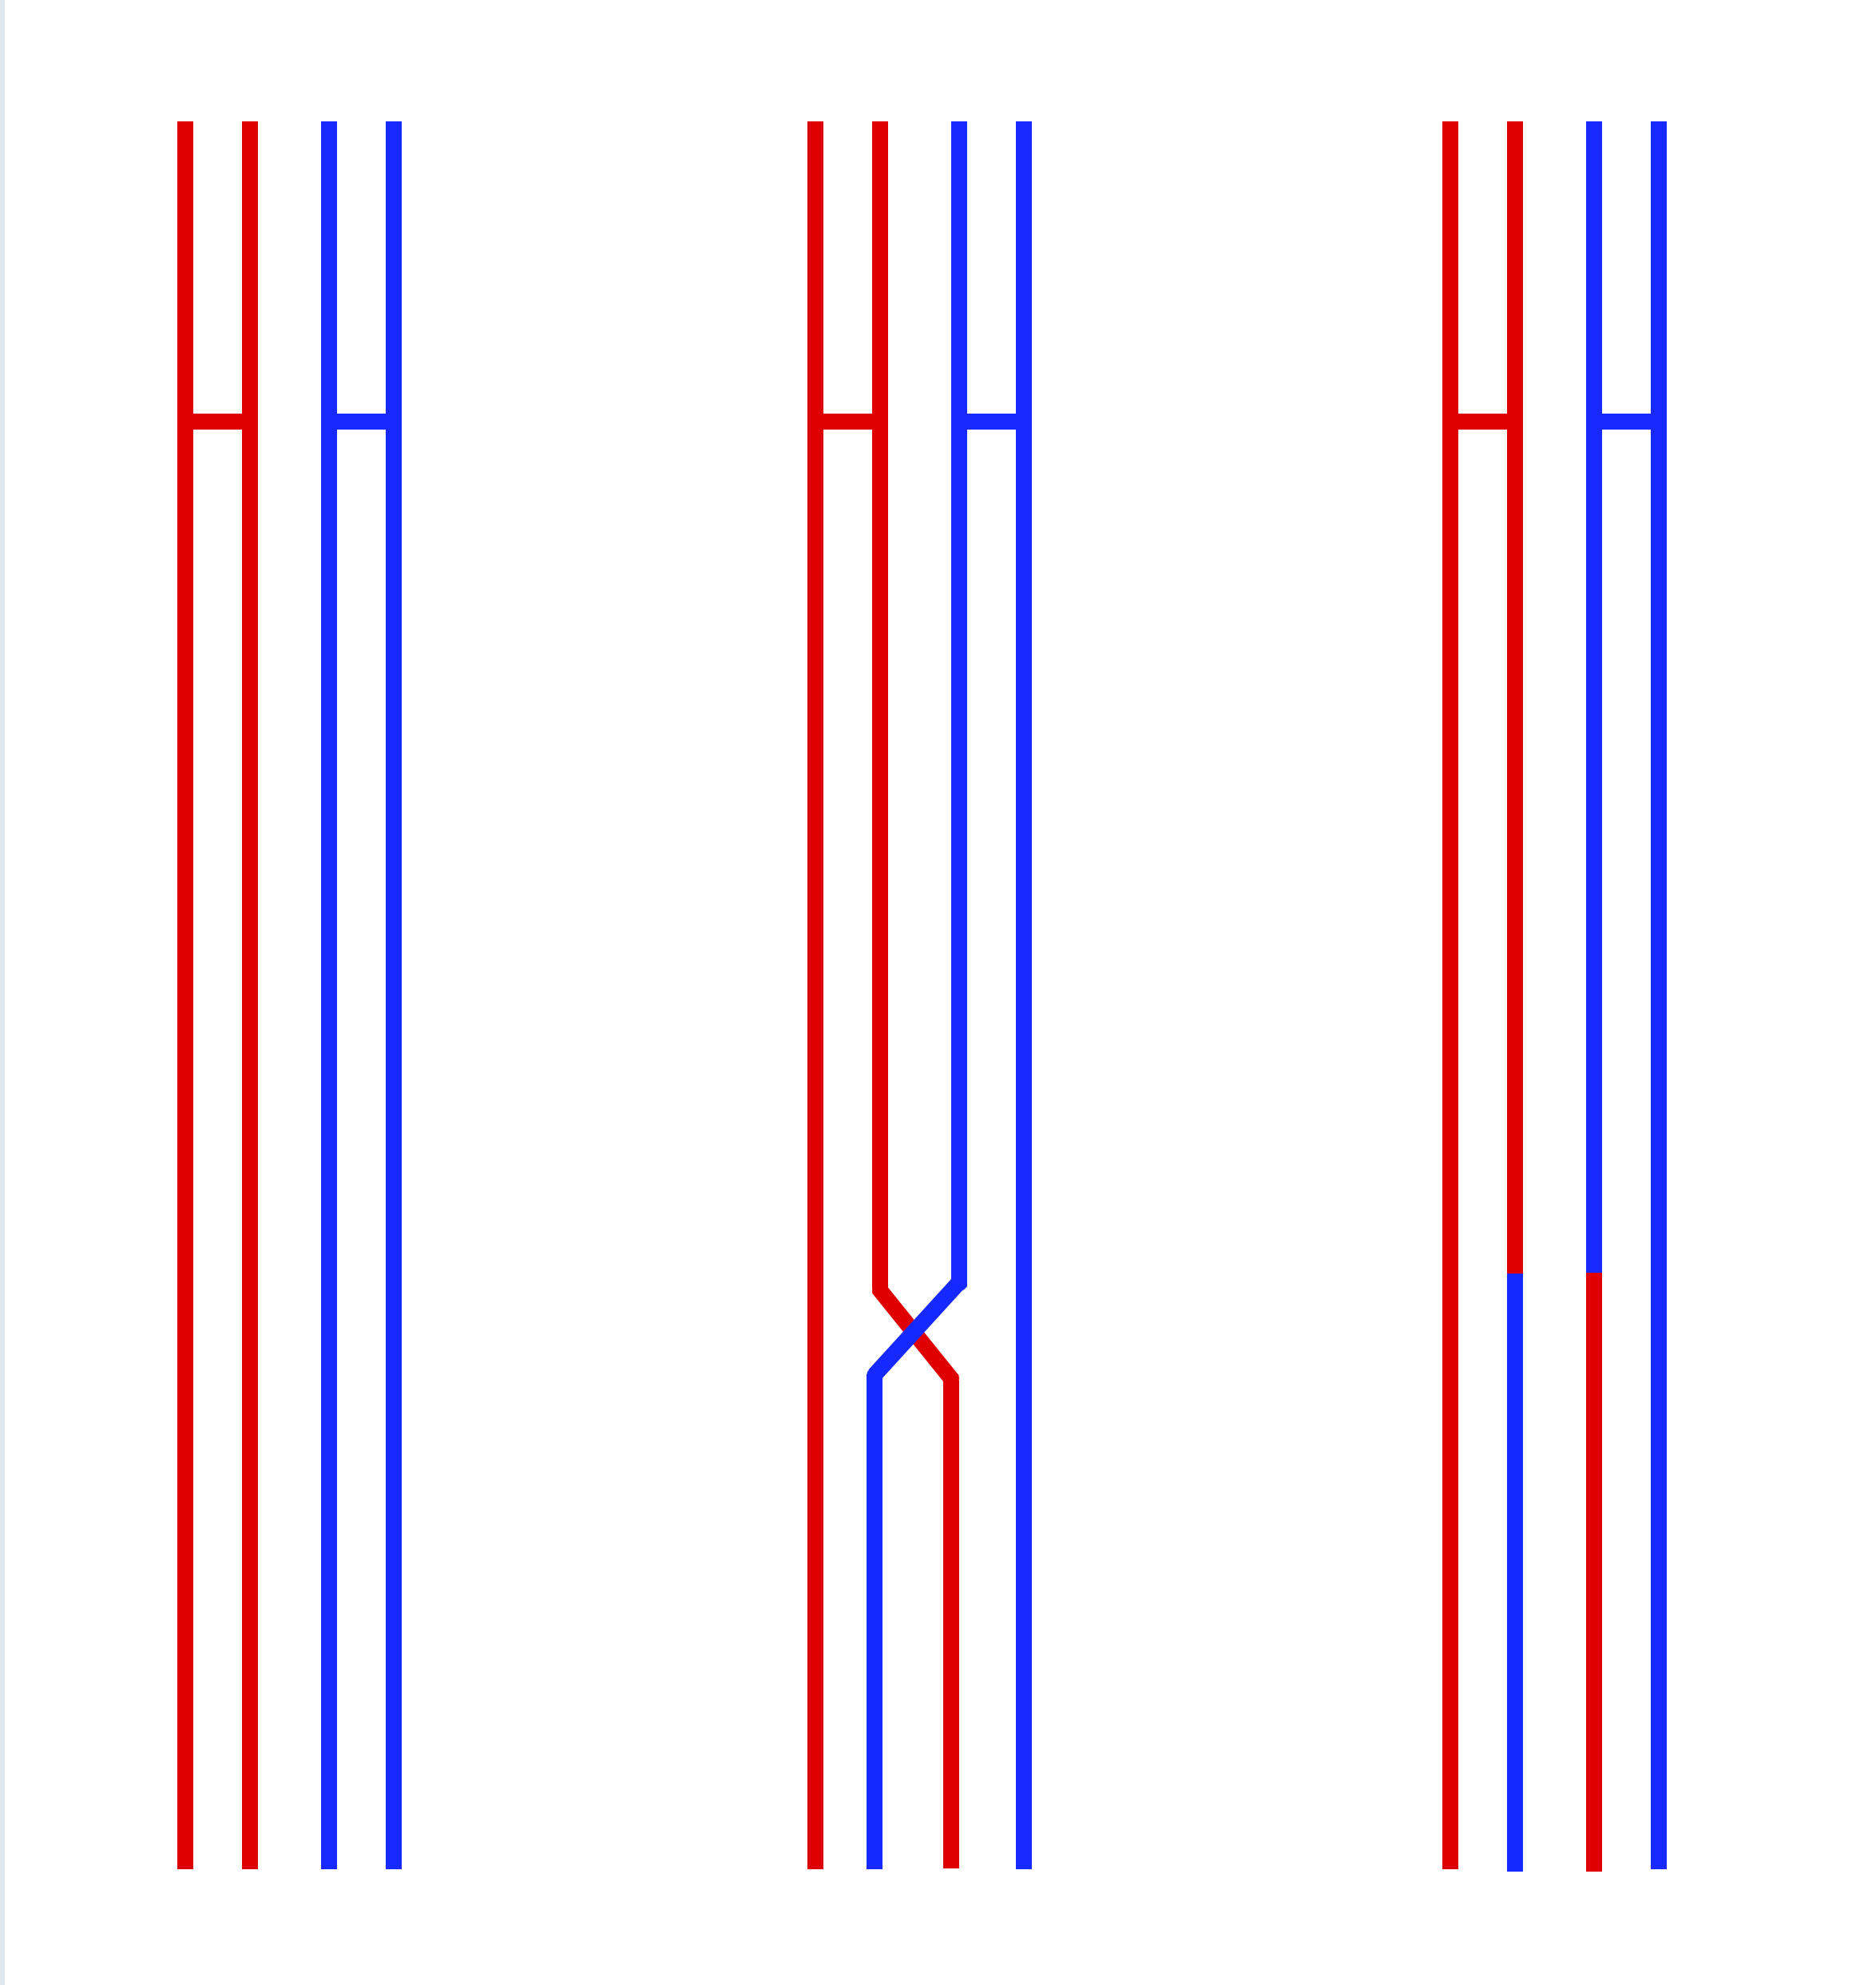
\includegraphics[width=0.7\textwidth]{img/crossing_over.jpg}}
		\caption{Profaza mejozy - crossing-over}
		\label{fig:crossingover}
\end{figure}

\subsection{Dobór naturalny}
    To czynnik nadający ewolucji kierunkowy i przystosowawczy charakter. Ma na celu zwiększenie stopnia przystosowania (adaptacji) do warunków środowiskowych 
zarówno na poziomie osobniczym jak i genowym.
 Organizmy posiadające korzystne cechy mają większą szansę na przeżycie 
i rozmnażanie, co prowadzi do zwiększania częstości występowania korzystnych genów 
w populacji.
\subsection{ Dryft genetyczny (zjawisko Wrighta) }
    Dryftem genetycznym nazywa się wahania częstotliwości występowania genu 
nie wynikające z działania doboru naturalnego, migracji, czy mutacji. Jest efektem losowych zmian w ilości alleli w kolejnych pokoleniach. ~\cite{encykBio}
 \subsection{ Hybrydyzacja (krzyżowanie) } ~\label{sec:hybryda}
Hybrydyzacja to proces polegający na krzyżowaniu się osobników, będących przedstawicielami różnych genetycznie populacji, w wyniku którego może powstać potomstwo mieszańcowe. Może to doprowadzić do powstania nowych gatunków, lub przyczynić się do zwiększenia różnorodności genetycznej populacji, bądź pojawienia się w populacji nowych korzystnych cech.~\cite{hybry}
\section{ Strategie ewolucyjne (ES) }
Pojęcie strategii ewolucyjnych powstało w latach pięćdziesiątych XX wieku, gdy naukowcy postawili sobie za cel wykorzystanie teorii ewolucji Darwina  oraz zasady doboru naturalnego na zbiorze potencjalnych wyników do ich optymalizacji.~\cite{javaGen} 
W 1975 roku profesor J.H. Holland jako pierwszy opracował koncept algorytmów genetycznych, które zaprezentowano w książce \enquote{\textit{Adaption in Natural and Artificial Systems}}. Zaproponował on, by zamodelować chromosomy w postaci ciągów zer i jedynek. Tak przygotowany zbiór wejściowy z łatwością ulegać może \enquote{ewolucji} poprzez mutację, selekcję, czy też crossing-over.~\cite{javaGen}
Słownik pojęć niezbędnych do poruszania się po temacie zaprezentowano w tabeli~\ref{table:dicTab} \begin{table}
\renewcommand\arraystretch{1.5}
 \centering
    \begin{tabular}{|>{\centering\arraybackslash}m{4cm}|m{8.5cm}|}
     \hline
    \textbf{Pojęcie} & \textbf{Objaśnienie}\\ \hline
     Chromosom& Zakodowana forma potencjalnego rozwiązania zadanego problemu. Ciąg uporządkowanych genów.\\ \hline 
     Gen & Element składowy chromosomu.  \\ \hline
    Osobnik & Dla algorytmów genetycznych, równoważny z pojęciem chromosomu. Niekiedy jednak prezentowany jako zespół chromosomów (genotyp).\\ \hline
     Fenotyp& Odpowiednik genotypu w przestrzeni odkodowanej. \\ \hline
     Populacja& Zbiór osobników o określonej liczebności.\\ \hline
     Przystosowanie& Przystosowanie osobników do zadanego problemu. Oceniane za pomocą funkcji przystosowania. Im większy stopień przystosowania, tym lepsze rozwiązanie. \\ \hline
     Selekcja & Proces filtracji najlepiej dopasowanych osobników spośród populacji. Wybrane chromosomy trafiają do populacji rodzicielskiej, przygotowywanej do rekombinacji genów.\\ \hline
     Krzyżowanie &  Rekombinacja genów chromosomów rodzicielskich, której wynikiem jest chromosom potomny o zmienionym składzie. Patrz ~\ref{sec:hybryda}  \\ \hline 
    Rodzic & Chromosom wybrany do krzyżowania. \\ \hline
    Potomek & Wynik krzyżowania pary rodziców. \\ \hline
    Mutacja & Proces zamiany genów w obrębie jednego chromosomu bez wpływu chromosomów rodzicielskich. Patrz ~\ref{sec:mutate}\\ \hline
	\end{tabular}
	 \caption{Słownik pojęć podstawowych} 
    \label{table:dicTab}
\end{table}


    \subsection{ Algorytm ewolucyjny (EA), Algorytm Genetyczny (GA)}
Algorytmem ewolucyjnym nazywamy algorytm probabilistyczny, opierający się na zasadach obowiązujących w ewolucji organicznej  ~\cite{genAlgWeb}, dla którego generowany jest zbiór osobników $P(t)=\lbrace x_1^t, ..., x_n^t\rbrace$ w każdej iteracji $t$. Każdy osobnik przedstawia potencjalne rozwiązanie zadanego problemu i posiada swoją reprezentację jako struktura danych S. Obiekty zbioru oceniane są w oparciu o ich \enquote{dopasowanie}. W iteracji $t+1$ tworzy się nową populację osobników. Jest ona wynikiem selekcji najlepiej \enquote{dopasowanych} obiektów z iteracji $t$. Niektóre z wybranych podlegają transformacji (mutacja / crossing-over) dając nowe rozwiązania. Po zakończeniu działania algorytmu oczekuje się, iż najlepsze możliwe osobniki znajdą się w zbiorze końcowym i reprezentują rozwiązanie znajdujące się blisko optymalnego (rozwiązanie rozsądne).[ ~\cite{algBook}] W ten sposób unika się przeszukiwania całej przestrzeni w poszukiwaniu rozwiązania, a wybierana zostaje jedynie niewielka populacja jej przedstawicieli. A dzięki mutacjom otrzymuje się rozwiązania coraz lepsze, bliskie optimum.  Ogólny schemat blokowy działania algorytmu przedstawiono na rysunku ~\ref{fig:algSchem}.

\begin{figure}[!h]
		\centering
		\scalebox{.8}{
		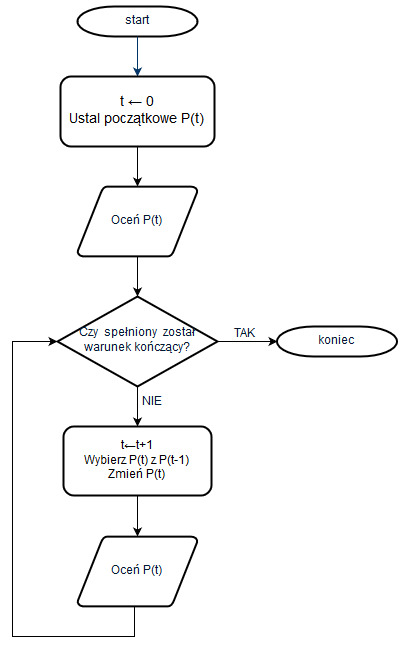
\includegraphics[width=0.7\textwidth]{img/program_ewolucyjny_alg.jpg}}
		\caption{Struktura programu ewolucyjnego}
		\label{fig:algSchem}
\end{figure}

Podczas  analizy literatury stwierdzono, iż nazwy \enquote{algorytm ewolucyjny}  oraz \enquote{algorytm  genetyczny} stosuje się zamiennie. W  poniższym tekście  przyjęto również taką koncepcję. 

\subsection{ Algorytm genetyczny a program ewolucyjny}
 Na podstawie algorytmów ewolucyjnych powstały programy ewolucyjne. Ich struktura pozostaje taka sama, jednak różnice widać na niższym poziomie. 
Dla algorytmów przyjęto zapis w postaci skończonego, uporządkowanego ciągu  jasno zdefiniowanych czynności, koniecznych do wykonania pewnego zadania. Konieczny do rozszyfrowania tego zapisu jest specjalny parser, który zamienia ciąg w wykonalną funkcję oraz rozpoznaje ewentualne zmiany stanu (wywołane mutacją, bądź crossing-over), które mogłyby zagrażać jego działaniu.  W porównaniu do tego program ewolucyjny jest przedstawiony jako  drzewiasta struktura czynności i wartości. Również niezbędny jest parser, jednak pomniejszony o świadomość stanów ( te ukryte są wewnątrz struktury). 
\\
Poza tym znaczącą różnicę stanowi reprezentacja chromosomów. Dla algorytmów ewolucyjnych/genetycznych chromosomy muszą być w formie binarnej, natomiast program pozwala nam na zdefiniowanie dowolnych struktur.
Z tym związane jest również zapotrzebowanie na wprowadzenie spersonalizowanych operatorów genetycznych, odpowiednich dla zadanej struktury i zadania, podczas gdy algorytmy korzystają z podstawowych operatorów.
\\
Algorytmy genetyczne wymagają modyfikacji zadania (przetworzenie na łańcuch binarny). Nie jest to zadaniem łatwym i niekiedy może wymagać użycia parserów, czy też algorytmów naprawy, np. reprezentacja indeksów liczby z zakresu od 1 - 5, możliwa jest dzięki 3 bitom. Jednak podczas procesu mutacji mogą powstać indeksy wykraczające poza zakres (6-8). Zmienienie ich wartości do zgodnych z zakresem wymaga użycia specjalnego algorytmu naprawy. 
Programy ewolucyjne, natomiast,  wymagają zmiany reprezentacji chromosomowej potencjalnych rozwiązań oraz wytworzenia odpowiednich operatorów genetycznych do działania na wytworzonych strukturach.  Zależności te w sposób schematyczny przedstawiono na rysunkach (rys.~\ref{fig:roznice_alg}, rys.~\ref{fig:roznice_prog}).
\begin{figure}[!h]
		\centering
		\scalebox{.8}{
		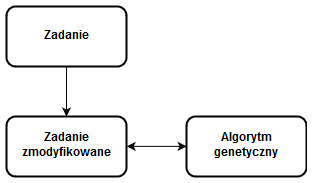
\includegraphics[width=0.7\textwidth]{img/schemat_alg_gen.jpg}}
		\caption{Schemat działania algorytmu genetycznego.}
		\label{fig:roznice_alg}
		\scalebox{.8}{
		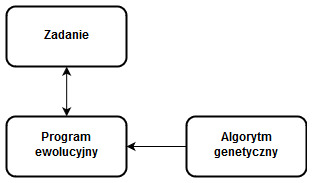
\includegraphics[width=0.7\textwidth]{img/schemat_prog_ew.jpg}}
		\caption{Schemat działania programu ewolucyjnego.}
		\label{fig:roznice_prog}
\end{figure}
\subsection{Wymagania}
Zarówno program jak i algorytm posiadają listę wymagań, które muszą zostać spełnione, by zapewnić ich poprawne działanie.~\cite{algBook}\\
Musi istnieć:
~\begin{itemize}
\item
zbiór z reprezentacją możliwych rozwiązań problemu,
\item
metoda generowania początkowej populacji potencjalnych rozwiązań, 
\item
funkcja oceniająca, do oceny \enquote{dopasowania} rozwiązań,
\item
operator \enquote{genetyczny} wpływający na populację,
\item
parametr populacji niezbędny algorytmowi (np. rozmiar populacji, prawdopodobieństwo mutacji, długość wykonywania się algorytmu itp.) 

\end{itemize}
\section{Ewolucyjne generowanie kodów źródłowych}
Tematem pracy jest implementacja programu, którego istotą jest generowanie kodów źródłowych programów  w sposób ewolucyjny, kierując się przy tym zadanym parametrem np. czasem wykonywania, czy długością kodu. Zagadnienie to w literaturze nazywane jest \enquote{\textit{automatic programming}}, czy też  \enquote{\textit{program synthesis}}  i określa wszelkie metody generowania kodów bez ingerencji człowieka mające na celu wytworzenie sprawnego oprogramowania na bazie określonej specyfikacji. 
\\ Zakłada się, iż istnieje następujący podział automatycznego programowania ~\cite{automaticProg} 
\begin{itemize}
\item Programowanie generatywne \\
	Powszechny rodzaj programowania, w którym biblioteki standardowe są wykorzystywane do poprawy jakości i prędkości oprogramowania. Programista nie musi samodzielnie implementować, ani znać sposobów działania niektórych funkcji, a jedynie skorzystać z gotowych rozwiązań biblioteki. 
\item Generowanie kodów źródłowych\\
 Kod źródłowy jest generowany na podstawie predefiniowanego modelu, czy wzorca, powstałego dzięki wykorzystaniu narzędzi programistycznych i odpowiedniego środowiska (IDE). Przykładem działania takiego programu jest \textit{Google/MIT App Inventor}, gdzie generuje się kod  na podstawie wzorca stworzonego przez użytkownika z bloków funkcji. Mechanizm ten nie wymaga od użytkownika napisania ani jednej linii kodu. 
\end{itemize}


\subsection{Dotychczasowe rozwiązania }
Podczas analizy literatury znaleziono kilka rozwiązań podobnych problemów, do zadanego w tej pracy. 
\subsubsection{Co-evolutionary automatic programming for software development} ~\label{sec:coEvo}
Jednym z ciekawszych rozwiązań, które udało się znaleźć jest podejście przedstawione w artykule ~\cite{coEvolution}. Zakłada ono wykorzystanie programowania genetycznego do ewolucji programów, podczas gdy testy jednostkowe, badające stopień dopasowania chromosomu wynikowego, ulegają  ko-ewolucji na zasadzie konkurencji. Dopasowanie programu (chromosomu) określane jest na podstawie ilości testów, które zwróciły wynik negatywny, natomiast dopasowanie testu wyliczane zostaje z ilości programów, które go nie przeszły. 
Zastosowano model drapieżnik - ofiara i przyjęto, że w roli drapieżnika stoją testy jednostkowe, natomiast ofiarą są programy. Jeśli program będzie zbyt \enquote{wolny} padnie ofiarą drapieżnika i nie przejdzie testu. Takie programy nie nadają się do dalszej ewolucji. Krzyżować się mogą jedynie osobnik \enquote{najszybsze}, w wyniku dając osobniki potomne, których zestaw cech powinien również gwarantować bezpieczeństwo przed drapieżnikiem. Gdyby testy (drapieżnicy) nie były objęte procesem ewolucji,  działanie programu ewoluującego szybko by się skończyło. By osiągnąć lepsze wyniki postanowiono ewoluować również populację testów. Testy o dużej skuteczności (tzn. wyszukujące dużą ilość niedziałających programów) przekazują swoje cechy dalej i pomagają tworzyć nowe testy, o ulepszonym działaniu. 
\\ Podczas działania algorytmu nie są porównywane wyniki otrzymanych programów z wynikiem przewidywanym (poprawnym), lecz jedynie  funkcja podobieństwa obu wyników, to jest odległość między wynikami. Jeśli jej wartość jest duża, to znaczy, że wyniki znacząco się miedzy sobą różnią i przeciwnie, w przypadku gdy odległość jest bliska zeru, wyniki można uznać za identyczne.  Dzięki temu nie jest konieczne przetrzymywanie informacji o tym, jaki wynik zwróci działanie programu, a jedynie wiadomość o jego względnej wartości w stosunku do wyniku poprawnego. 
\\  O ile istnieje możliwość wytworzenia formalnej specyfikacji, by wygenerować ciągłą funkcję dopasowania, to możliwe jest automatyczne wytworzenie programu. Przy czym wytworzenie poprawnie działającego programu  do rozwiązywania problemu stopu  ~\cite{algHalt} nie jest możliwe. 
\subsubsection{Automatic Generation of Programs using Genetic Network Programming} 
Praca ~\citep{networkProg}, w porównaniu do powyższego podejścia, nie skupiła się na ewoluowaniu testów podczas generowania programów, lecz na przetwarzaniu problemu za pomocą struktury sieci skierowanej. Udowodniono poprawę jakości w stosunku do zwykłego programowania genetycznego. \\
Sieć oparta jest na dwóch rodzajach węzłów : oceniających oraz przetwarzających.  Prócz tego istnieją również węzeł startu do inicjalizacji programu, pamięć współdzielona między węzłami oraz połączenia między węzłami przetwarzającymi.  Program działa według następującego algorytmu: 
\begin{enumerate}
\item Inicjalizuj losowo populację wejściową 
\item Wykonaj i oceń programy
\item Ewoluuj programy 
\begin{itemize}
\item Crossover - Wybierz dwóch rodziców i dowolny węzeł, dokonaj zamiany.
\item  Mutacja - Wybierz jednego rodzica i losowo zamień połączenia. 
\item Zachowanie elity  - Wybierz najlepszego osobnika i zachowaj jako potomka. 
\end{itemize}
\item Zastąp rodziców potomstwem. 
\item Powtarzaj kroki 2-4 aż nastąpi spełnienie warunku końcowego.

Węzeł przetwarzający na podstawie danych zawartych w pamięci wytwarza kod, który zapisuje do pamięci. Węzły oceniające, korzystając z funkcji dopasowania, oceniają węzły przetwarzające i koordynują, do którego z nich należy przejść w kolejnym kroku. 
\end{enumerate}
\subsubsection{Automatic Programming Using Genetic Programming}
Inne podejście można było zaobserwować w ~\cite{ownLanguage}. Autorzy stworzyli własny pseudo język programowania, który miał uprościć działanie programu genetycznego, a także zapewnić uniwersalność, tzn. wygenerowany kod może zostać przetłumaczony na dowolny język programowania. Liczba funkcji została ograniczona i zdefiniowana (tabla ~\ref{table:comendTabel}).
\begin{table}
\renewcommand\arraystretch{1.5}
 \centering
    \begin{tabular}{|M{4cm}|M{4cm}|M{4cm}|}
     \hline
    \textbf{Typ operacji} & \textbf{Funkcja}& \textbf{Ilość przyjmowanych parametrów}\\ \hline
      Arytmetyczna & $+,-,*,/$ &2 \\ \hline
     String & strequal, strnotequal &2 \\ \hline
     Logiczna & ==,!=,<=,>=,<,> & 2 \\ \hline
     Działania na pamięci & Write, Change, Read & 3,2,1\\ \hline
     Warunkowa & If, switchc,switchi & 3, $3\leqslant n \leqslant 8$\\ \hline
     Iteracja & For, While & 3, 2\\ \hline
     Wyrażenia złożone & block, n=2,3 , combn & 2 lub 3 ,$ 1\leqslant  n \leqslant 5$ \\ \hline

	\end{tabular}
	 \caption{Pseudo-język stworzony w artykule ~\cite{ownLanguage}}. 
    \label{table:comendTabel}
\end{table}
Samo działanie programu zachodzi natomiast w następujących krokach: 
\begin{enumerate}
\item Generowanie populacji początkowej \\
Każdy z osobników przedstawiony jest jako drzewo wyprowadzenia ~\citep{parsetree}.
\item Selekcja i ewaluacja \\
Wybierana jest para rodziców w procederze turnieju, tzn. z losowego zbioru kandydatów wybierane zostają osobniki o najlepszym dopasowaniu. Tak jak w artykule ~\ref{sec:coEvo} dopasowanie jest miarą odległości otrzymanego wyniku, do wyniku przewidywanego. Dla typu string sprawdzana jest ilość pokrywających się znaków (\textit{\enquote{ hits ratio}}).
\item Regeneracja\\
Dzięki operatorom genetycznym tworzeni są potomkowie wybranych rodziców. Mutacje polegają na wygenerowaniu nowego poddrzewa w wylosowanym węźle. Dla crossing-over zachodzi zamiana poddrzew miedzy dwoma rodzicami w wybranym węźle. 
\item Modularyzacja \\
Modularyzacja jest koncepcją mającą za zadanie podział drzewa na takie bloki, by wymiana informacji miedzy nimi była znacznie rzadsza niż wewnątrz. Poza tym zauważa się kompresję drzewa, przy jednoczesnym zachowaniu struktury. Poddrzewa są łączone, a w ich miejsca są dodawane etykiety. Dobre bloki funkcji (tzn. dające dobre wyniki) dodawane są do zestawu funkcji, co powoduje stopniowe uczenie się programu genetycznego. Głównym celem jest wiec rozłożenie zadanego problemu na prostsze - mniejsze, łatwiejsze do rozwiązania. 
\end{enumerate}
Autorzy artykułu przetestowali program dla 10 problemów i otrzymali zadowalające wyniki, zarówno jeśli chodzi o poprawność wyników, jak i czas pracy programów.  W dwóch problemach wyjątkowo skuteczna i niezbędna okazała się modularyzacja. 
\section{Podsumowanie}
   \end{document} 